The new scenario we have to consider is the one in which not all the parameters are known: here the conversion rates of the customers and the features of our customers are unknown, so our web site is not able to distinguish one from another. 

\subsection{Results}
\subsubsection{UCB}
\begin{figure}[ht]
    \begin{center}
    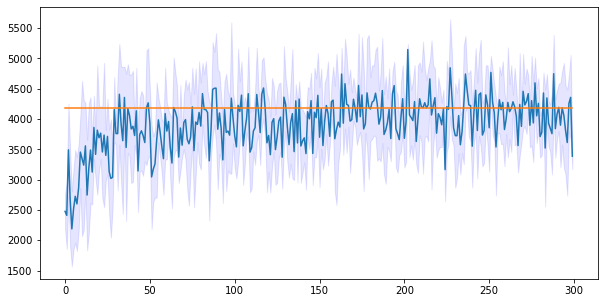
\includegraphics[width=0.6\textwidth]{img/ucb3.png}
    \caption{UCB Reward}
    \label{fig:reward31}
    \end{center}
\end{figure}
\begin{multicols}{2}
    \begin{figure}[H]
        \begin{center}
        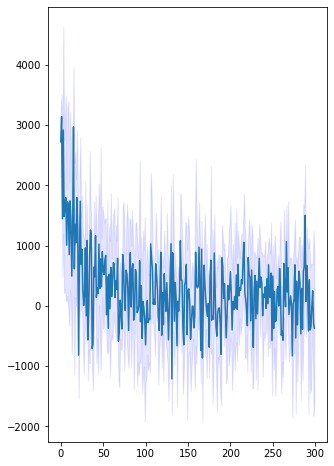
\includegraphics[width=0.5\textwidth]{img/ucb3_regret.png}
        \caption{UCB Regret}
        \label{fig:regret31}
        \end{center}
    \end{figure}
    \columnbreak
    \begin{figure}[H]
        \begin{center}
        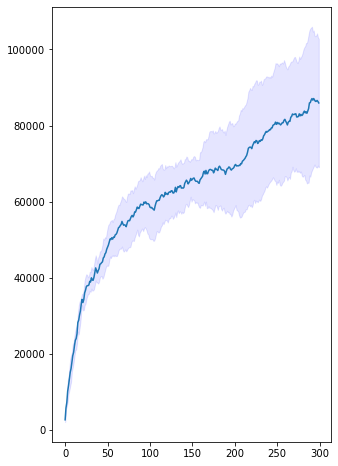
\includegraphics[width=0.5\textwidth]{img/ucb3_cum_reg.png}
        \caption{UCB Cumulative regret}
        \label{fig:cum_reg31}
        \end{center}
    \end{figure}
\end{multicols}
\subsubsection{TS}
\begin{figure}[ht]
    \begin{center}
    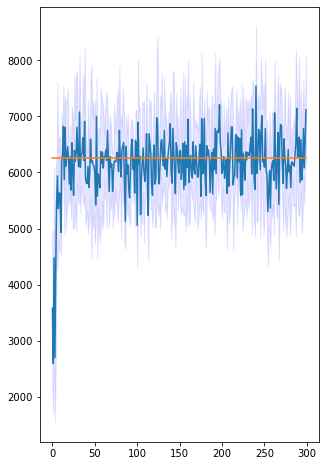
\includegraphics[width=0.6\textwidth]{img/TS3.png}
    \caption{TS Reward}
    \label{fig:reward32}
    \end{center}
\end{figure}
\begin{multicols}{2}
    \begin{figure}[H]
        \begin{center}
        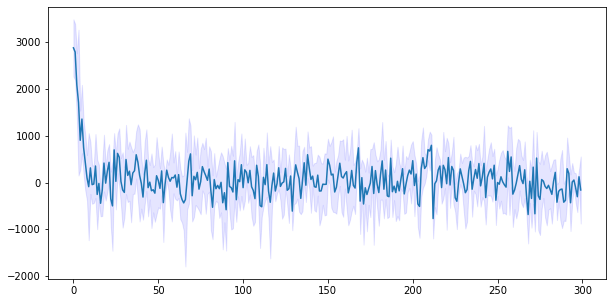
\includegraphics[width=0.5\textwidth]{img/TS3_regret.png}
        \caption{TS Regret}
        \label{fig:regret32}
        \end{center}
    \end{figure}
    \columnbreak
    \begin{figure}[H]
        \begin{center}
        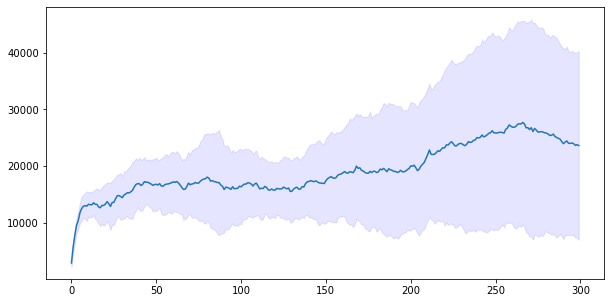
\includegraphics[width=0.5\textwidth]{img/TS3_cum_reg.png}
        \caption{TS Cumulative regret}
        \label{fig:cum_reg32}
        \end{center}
    \end{figure}
\end{multicols}